\chapter{有限差分法}
上一章推导的控制方程的解析解,如果可以得出,将可以给出所有因变量在求解域上连续函
数。然而,除了个别极其简单的流动情况,这类方程的解析解往往很难获得。因此,我们只
能退而求其次,通过将连续的空间和时间分割成不连续的散点(分别称为网格点和时间节点
),并将控制方程在这些散点上离散,得出与原方程近似但可求解的代数方程组,最终得出
原方程在这些散点上的近似解。

在实际的数值模拟过程中,网格点或时间节点的划分是不均匀的。为了后续推导方便,本章
假定网格点和时间节点的间距都是均匀分布的。此外,本章只关注结构网格,对非结构网格
可参见其他参考书。

\section{泰勒展开}
考虑一个$x$的连续函数$f(x)$在$x$处的所有阶导数都存在。那么,$f$在点$x+\Delta x$
处的值可以通过在点$x$处的泰勒级数展开来估算。
\begin{equation}
  f(x+\Delta x)
  =
  f(x)
  +
  \frac{\mathrm{d} f}{\mathrm{d} x}\Delta x
  +
  \frac{\mathrm{d}^{2} f}{\mathrm{d} x^{2}}\frac{\Delta x^{2}}{2}
  +
  \cdots
  +
  \frac{\mathrm{d}^{n} f}{\mathrm{d} x^{n}}\frac{\Delta x^{n}}{n!}
  +
  \cdots
\end{equation}

假定$f(x)=\sin{2\pi x}$,且已知$x=0.2$处,函数值$f=0.9511$。我们希望估算
$x+\Delta x=0.22$处的函数值。根据方程表达式,该点的精确值为0.9823。首先,我们利
用泰勒级数展开的第一项来估算,有
\begin{equation}
  \begin{aligned}
    f(x+\Delta x) \approx f(x)  \\
    f(0.22) \approx f(0.2) = 0.9511
  \end{aligned} 
\end{equation}
估算值的相对误差为$(0.9823-0.9511)/0.9823=3.176\%$。接着,我们利用展开式的前两项
来估算,有
\begin{equation}
  \begin{aligned}
    f(x+\Delta x) &\approx f(x) + \frac{\mathrm{d} f}{\mathrm{d} x}\Delta x
  \\
    f(0.22) &\approx f(0.2) + 2\pi\cos{[2\pi(0.2)]}(0.02)
    \\
            &\approx 0.9511 + 0.388 = 0.9899
\end{aligned}
\end{equation}
估算值的相对误差为$(0.9899-0.9823)/0.9823=0.775\%$,相比于第一次的估算值更加接近
精确值。最后,为了获得更加精确的估算值,我们可以利用展开式的前三项,有
\begin{equation}
  \begin{aligned}
    f(x+\Delta x) &\approx f(x) + \frac{\mathrm{d} f}{\mathrm{d} x}\Delta x
    +
    \frac{\mathrm{d}^{2} f}{\mathrm{d} x^{2}}\frac{(\Delta x)^{2}}{2}
  \\
    f(0.22) &\approx f(0.2) + 2\pi\cos{[2\pi(0.2)]}(0.02) -
    4\pi^{2}\sin{[2\pi(0.2)]}\frac{0.02^{2}}{2}
    \\
            &\approx 0.9511 + 0.0388 - 0.0075
    \\
            &\approx 0.9824
\end{aligned}
\end{equation}
估算值的相对误差为$(0.9824-0.9823)/0.9823=0.01\%$,即仅用泰勒展开式的前三项就可
以得到一个非常接近精确值的估算值。

\section{离散基础知识}
图\ref{FgBD_SMN}中给出了一个结构网格的例子。图中,网格点,即两条网格线的交点,可以用$(i,j)$进
行标示,其中,$i$是沿$x$方向的索引,$j$是沿$y$方向的索引。假定图中$P$的索引为
$(i,j)$,那么,紧邻$P$右边的点的索引为$(i+1,j)$,紧邻$P$左边的点的索引为
$(i-1,j)$,紧邻$P$上边的点的索引为$(i,j+1)$,紧邻$P$下边的点的索引为$(i,j-1)$。
对非恒定流中,离散的当前时间层用上标$n$来标记,下一个时间层用上标$n+1$来标记,前
一个时间层用上标$n-1$来标记。
\begin{figure}[ht]
  \centering
  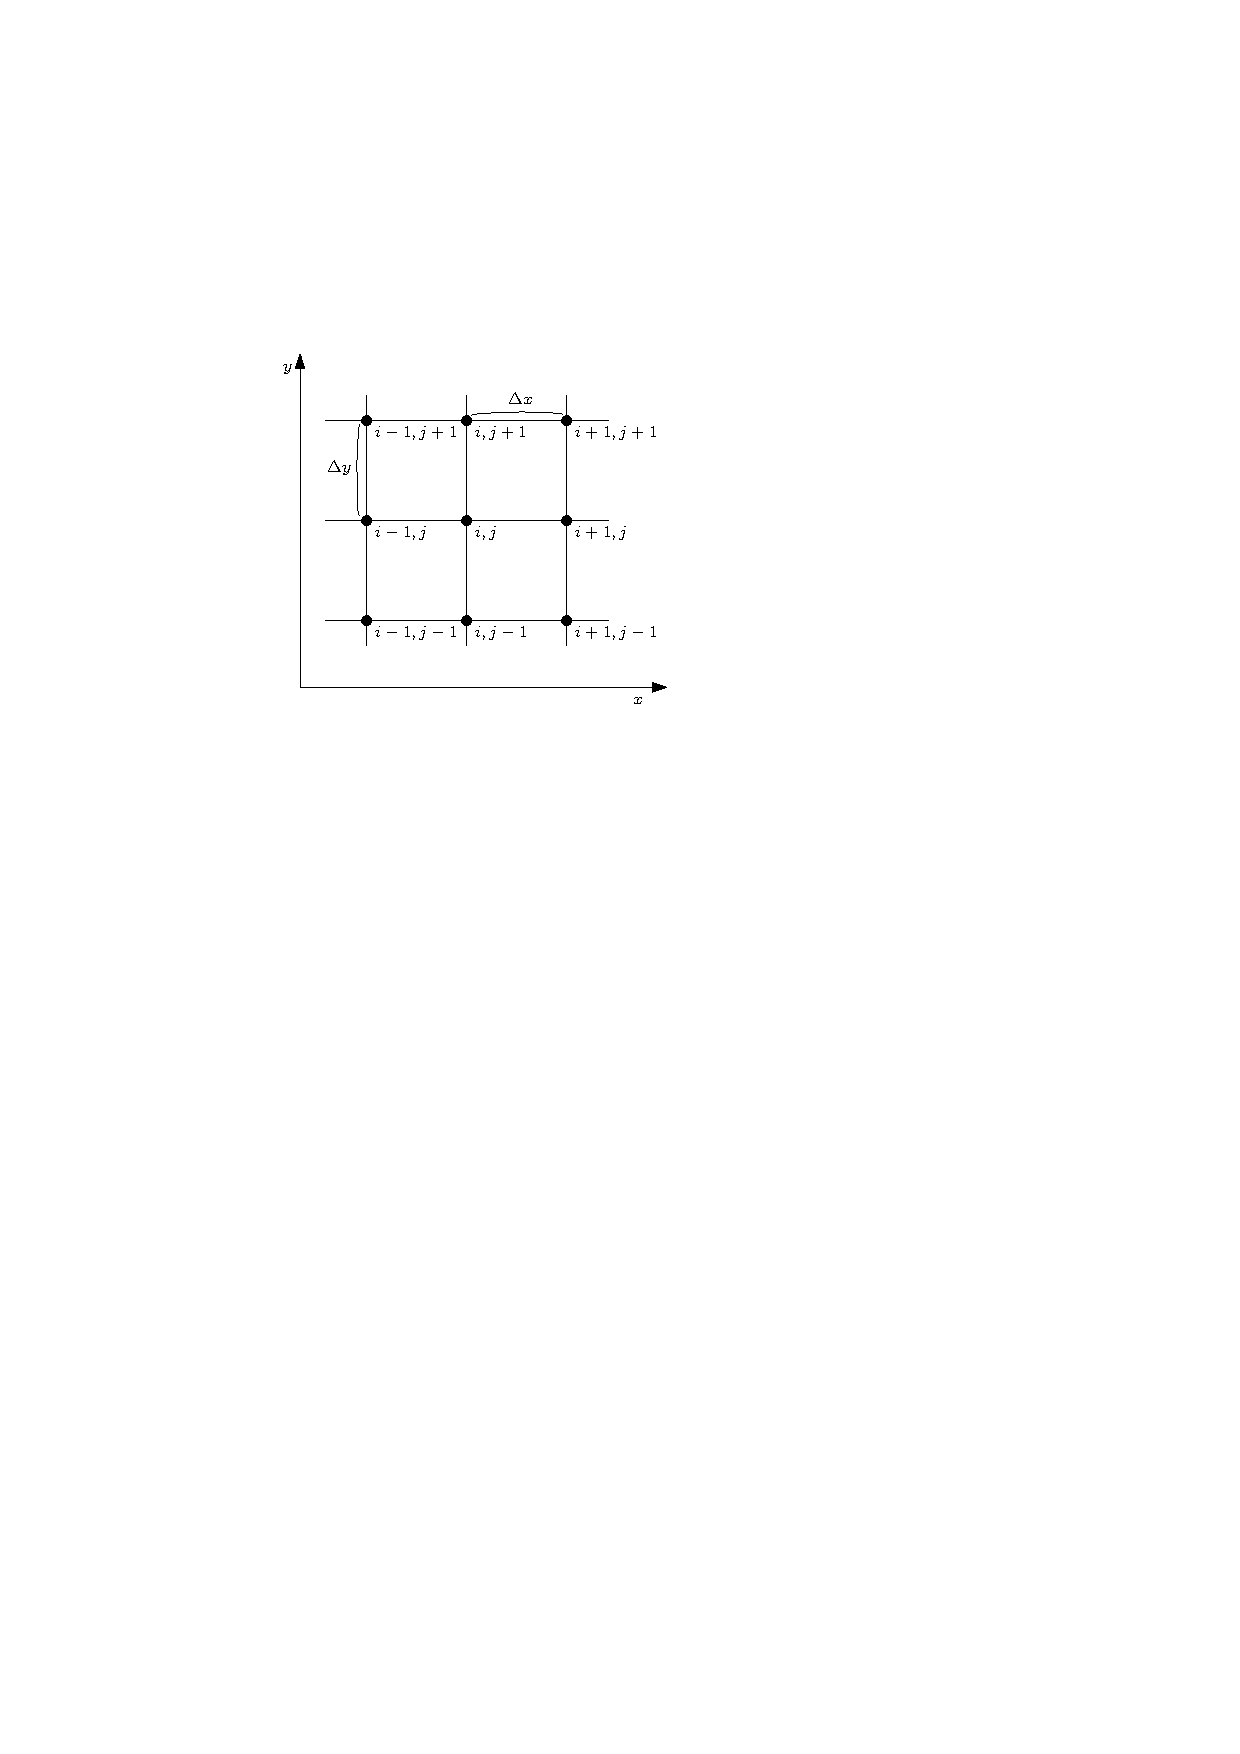
\includegraphics{BDStructureMeshNotion.pdf}
  \caption{结构网格离散网格节点示意}
  \label{FgBD_SMN}
\end{figure}

\subsection{一阶偏导数的差分表达式}
点$(i,j)$上$x$方向速度用$u_{i,j}$表示,点$(i+1,j)$上$x$方向速度$u_{i+1,j}$可以在
点$(i,j)$上通过泰勒级数展开为:
\begin{equation}
  u_{i+1,j}
  =
  u_{i,j} + 
  \left(
    \frac{\partial u}{\partial x}
  \right)_{i,j}
  \Delta x
  +
  \left(
    \frac{\partial^{2} u}{\partial x^{2}}
  \right)_{i,j}
  \frac{(\Delta x)^{2}}{2}
  +
  \left(
    \frac{\partial^{3} u}{\partial x^{3}}
  \right)_{i,j}
  \frac{(\Delta x)^{3}}{3!}
  +
  \cdots
  \label{EqBD_Tsp_F}
\end{equation}
用上式求解$(\partial u/\partial x)_{i,j}$,可得
\begin{equation}
  \left(
    \frac{\partial u}{\partial x}
  \right)_{i,j}
  =
  \underbrace{
  \frac{u_{i+1,j}-u_{i,j}}{\Delta x}
}_{\mbox{差分表达式}}
  -
  \underbrace{
  \left(
    \frac{\partial^{2} u}{\partial x^{2}}
  \right)_{i,j}
  \frac{\Delta x}{2}
  -
  \left(
    \frac{\partial^{3} u}{\partial x^{3}}
  \right)_{i,j}
  \frac{(\Delta x)^{2}}{6}
  +
  \cdots
}_{\mbox{截断误差}}
\label{EqBD_Tes}
\end{equation}
上式中,如果我们用等号右边的差商$(u_{i+1,j}-u_{i,j})/\Delta x$来近似
$(\partial u/\partial x)_{i,j}$,则该项为偏导数的差分表达式,等号右边的其他项为截断误
差,可以省略。即,
\begin{equation}
  \left(
    \frac{\partial u}{\partial x}
  \right)_{i,j}
  \approx
  \frac{u_{i+1,j}-u_{i,j}}{\Delta x}
\end{equation}

式\eqref{EqBD_Tes}也可写成
\begin{equation}
  \left(
    \frac{\partial u}{\partial x}
  \right)_{i,j}
  =
  \frac{u_{i+1,j}-u_{i,j}}{\Delta x}
  +
  O(\Delta x)
  \label{EqBD_1P1AF}
\end{equation}
从上式可看出,被省略的截断误差中$\Delta x$的幂次最小的那一项决定了上式的精度
。截断误差中$\Delta x$的幂次即为式\eqref{EqBD_1P1AF}的精度。上式中截断误差中
$\Delta x$的最小幂次为1。因而,式\eqref{EqBD_1P1AF}为一阶精度,此外,式\eqref{EqBD_1P1AF}
中差分表达式使用了网格点$(i,j)$及其右侧相邻网格点$(i+1,j)$的信息,没有使用
$(i,j)$左侧网格点信息。因此,式\eqref{EqBD_1P1AF}也叫做向前差分。综上,式
\eqref{EqBD_1P1AF}为一阶偏导数$(\partial u/\partial x)_{i,j}$的一阶向前差分。

同理,$u_{i-1,j}$在$(i,j)$上进行泰勒级数展开为
\begin{equation}
  u_{i-1,j}
  =
  u_{i,j} - 
  \left(
    \frac{\partial u}{\partial x}
  \right)_{i,j}
  \Delta x
  +
  \left(
    \frac{\partial^{2} u}{\partial x^{2}}
  \right)_{i,j}
  \frac{(\Delta x)^{2}}{2}
  -
  \left(
    \frac{\partial^{3} u}{\partial x^{3}}
  \right)_{i,j}
  \frac{(\Delta x)^{3}}{3!}
  +
  \cdots
  \label{EqBD_Tsp_B}
\end{equation}
利用上式求解$(\partial u/\partial x)_{i,j}$,得
\begin{equation}
  \left(
    \frac{\partial u}{\partial x}
  \right)_{i,j}
  =
  \frac{u_{i,j}-u_{i-1,j}}{\Delta x}
  +
  O(\Delta x)
  \label{EqBD_1P1AB}
\end{equation}
上式中没有使用网格点$(i,j)$右侧网格点信息。因而,式\eqref{EqBD_1P1AB}为向后差分
。此外,上式中,截断误差中$\Delta x$的最低幂次为1。因此,式\eqref{EqBD_1P1AB}为
一阶偏导数$(\partial u/\partial x)_{i,j}$的一阶向后差分。

在计算水动力学、计算流体力学的实际应用中,一阶精度往往是不够的。为了构造一个二阶
精度的差分,将式\eqref{EqBD_Tsp_B}从式\eqref{EqBD_Tsp_F}中减去:
\begin{equation}
  u_{i+1,j} - u_{i-1,j}
  =
  2
  \left(
    \frac{\partial u}{\partial x}
  \right)_{i,j}
  \Delta x
  +
  2
  \left(
    \frac{\partial^3 u}{\partial x^3}
  \right)_{i,j}
  \frac{(\Delta x)^3}{3!}
  +
  \cdots
\end{equation}
上式可写成
\begin{equation}
  \left(
    \frac{\partial u}{\partial x}
  \right)_{i,j}
  =
  \frac{u_{i+1,j} - u_{i-1,j}}{2\Delta x}
  +
  O[(\Delta x)^{2}]
  \label{EqBD_1P2AC}
\end{equation}
式\eqref{EqBD_1P2AC}中使用了点$(i,j)$两侧节点$(i+1,j)$和$(i-1,j)$的信息。另外,
式\eqref{EqBD_1P2AC}中截断误差的最低幂次为2。因此,式\eqref{EqBD_1P2AC}是一阶偏
导数$(\partial u/\partial x)_{i,j}$的二阶中心差分。

同理,可以得到一阶偏导数$(\partial u/\partial y)_{i,j}$和
$(\partial u/\partial t)_{i,j}$
的差分格式。总结如下:
\begin{equation}
  \left(
    \frac{\partial u}{\partial x}
  \right)_{i,j}
  =
  \left\{
    \begin{aligned}
      &\frac{u_{i+1,j}-u_{i,j}}{\Delta x} + O(\Delta x) & \mbox{一阶向前差分} \\
      &\frac{u_{i,j}-u_{i-1,j}}{\Delta x} + O(\Delta x) & \mbox{一阶向后差分} \\
      &\frac{u_{i+1,j}-u_{i-1,j}}{2\Delta x} + O[(\Delta x)^{2}] \quad& \mbox{二阶中心差分} \\
    \end{aligned}
  \right.
\end{equation}

\begin{equation}
  \left(
    \frac{\partial u}{\partial y}
  \right)_{i,j}
  =
  \left\{
    \begin{aligned}
      &\frac{u_{i,j+1}-u_{i,j}}{\Delta y} + O(\Delta y) & \mbox{一阶向前差分} \\
      &\frac{u_{i,j}-u_{i,j-1}}{\Delta y} + O(\Delta y) & \mbox{一阶向后差分} \\
      &\frac{u_{i,j+1}-u_{i,j-1}}{2\Delta y} + O[(\Delta y)^{2}] \quad& \mbox{二阶中心差分} \\
    \end{aligned}
  \right.
\end{equation}

\begin{equation}
  \left(
    \frac{\partial u}{\partial t}
  \right)_{i,j}^{n}
  =
  \left\{
    \begin{aligned}
      &\frac{u_{i,j}^{n+1}-u_{i,j}^{n}}{\Delta t} + O(\Delta t) & \mbox{一阶向前差分} \\
      &\frac{u_{i,j}^{n}-u_{i,j}^{n-1}}{\Delta t} + O(\Delta t) & \mbox{一阶向后差分} \\
      &\frac{u_{i,j}^{n+1}-u_{i,j}^{n-1}}{2\Delta t} + O[(\Delta t)^{2}] \quad& \mbox{二阶中心差分} \\
    \end{aligned}
  \right.
\end{equation}


\subsection{二阶偏导数的差分表达式}
将式\eqref{EqBD_Tsp_F}和式\eqref{EqBD_Tsp_B}相加,可得
\begin{equation}
  u_{i+1,j} + u_{i-1,j}
  =
  2u_{i,j}+
  \left(
    \frac{\partial^{2} u}{\partial x^{2}}
  \right)_{i,j}(\Delta x)^{2}
  +
  \left(
    \frac{\partial^{4} u}{\partial x^{4}}
  \right)_{i,j}\frac{(\Delta x)^{4}}{12}
  +
  \cdots
\end{equation}
利用上式求解出$(\partial^{2}u/\partial x^{2})_{i,j}$,
\begin{equation}
  \left(
    \frac{\partial^{2} u}{\partial x^{2}} 
  \right)_{i,j}
  =
  \frac{u_{i+1,j}-2u_{i,j}+u_{i-1,j}}{(\Delta x)^{2}}
  +
  O[(\Delta x)^{2}]
  \label{EqBD_2P2AC}
\end{equation}
式\eqref{EqBD_2P2AC}中,等号右边第一项是二阶偏导数$(\partial^{2}u/\partial x^{2})_{i,j}$的中心差分
截断误差中$\Delta x$的最小幂次为2,因此该式为二阶精度。同理,我们可以得到
$(\partial^{2}u/\partial y^{2})_{i,j}$的二阶精度中心差分,
\begin{equation}
  \left(
    \frac{\partial^{2} u}{\partial y^{2}} 
  \right)_{i,j}
  =
  \frac{u_{i,j+1}-2u_{i,j}+u_{i,j-1}}{(\Delta y)^{2}}
  +
  O[(\Delta y)^{2}]
  \label{EqBD_2Py2AC}
\end{equation}

对于二阶混合偏导,如$\partial^{2} u/\partial x\partial y$,可以采用与上面类似的
处理方式得到。首先,将式\eqref{EqBD_Tsp_F}对$y$求偏导,得
\begin{equation}
  \left(
    \frac{\partial u}{\partial y}
  \right)_{i+1,j}
  =
  \left(
    \frac{\partial u}{\partial y}
  \right)_{i,j}
  +
  \left(
    \frac{\partial^{2} u}{\partial x\partial y}
  \right)_{i,j}\Delta x
  +
  \left(
    \frac{\partial^{3} u}{\partial x^{2}\partial y}
  \right)_{i,j}\frac{(\Delta x)^{2}}{2} 
  +
  \left(
    \frac{\partial^{4} u}{\partial x^{3}\partial y}
  \right)_{i,j}\frac{(\Delta x)^{3}}{6} 
  +
  \cdots
  \label{EqBD_Tsp_F_py}
\end{equation}
然后,将式\eqref{EqBD_Tsp_B}对$y$求偏导,得
\begin{equation}
  \left(
    \frac{\partial u}{\partial y}
  \right)_{i-1,j}
  =
  \left(
    \frac{\partial u}{\partial y}
  \right)_{i,j}
  -
  \left(
    \frac{\partial^{2} u}{\partial x\partial y}
  \right)_{i,j}\Delta x
  +
  \left(
    \frac{\partial^{3} u}{\partial x^{2}\partial y}
  \right)_{i,j}\frac{(\Delta x)^{2}}{2} 
  -
  \left(
    \frac{\partial^{4} u}{\partial x^{3}\partial y}
  \right)_{i,j}\frac{(\Delta x)^{3}}{6} 
  +
  \cdots
  \label{EqBD_Tsp_B_py}
\end{equation}
将式\eqref{EqBD_Tsp_F_py}中减去式\eqref{EqBD_Tsp_B_py},得
\begin{equation}
  \left(
    \frac{\partial u}{\partial y}
  \right)_{i+1,j}
  -
  \left(
    \frac{\partial u}{\partial y}
  \right)_{i-1,j}
  =
  2
  \left(
    \frac{\partial^{2} u}{\partial x\partial y}
  \right)_{i,j}\Delta x
  +
  \left(
    \frac{\partial^{4} u}{\partial x^{3}\partial y}
  \right)_{i,j}\frac{(\Delta x)^{3}}{3} 
  +
  \cdots
\end{equation}
从上式中求解$(\partial^{2}u/\partial x\partial y)$,得
\begin{equation}
  \left(
    \frac{\partial^{2} u}{\partial x\partial y}
  \right)_{i,j}
  =
  \frac{(\partial u/\partial y)_{i+1,j}-(\partial u/\partial y)_{i-1,j}}{2\Delta x}
  -
  \left(
    \frac{\partial^{4} u}{\partial x^{3}\partial y}
  \right)_{i,j}\frac{(\Delta x)^{3}}{6} 
  +
  \cdots
  \label{EqBD_2PM2A}
\end{equation}
上式中等式右侧第一项中需要求解$(\partial u/\partial y)_{i+1,j}$和$(\partial
u/\partial y)_{i-1,j}$。利用上一小节所得到一阶偏导数的中心差分,得
\begin{equation}
  \left(
    \frac{\partial u}{\partial y}
  \right)_{i+1,j}
  =
  \frac{u_{i+1,j+1}-2u_{i+1,j}-u_{i+1,j-1}}{2\Delta y} + O[(\Delta y)^{2}]
\end{equation}
\begin{equation}
  \left(
    \frac{\partial u}{\partial y}
  \right)_{i-1,j}
  =
\frac{u_{i-1,j+1}-2u_{i-1,j}-u_{i-1,j-1}}{2\Delta y} + O[(\Delta y)^{2}]
\end{equation}
将上两式代入式\eqref{EqBD_2PM2A},可得
\begin{equation}
  \left(
    \frac{\partial^{2} u}{\partial x\partial y}
  \right)_{i,j}
  =
  \frac{u_{i+1,j+1}-u_{i+1,j-1}-u_{i-1,j+1}+u_{i-1,j-1}}{4\Delta x\Delta y}
  +
  O[(\Delta x)^{2},(\Delta y)^{2}]
\end{equation}

本节所列出的差分格式只是所有差分格式的一小部分。同一个导数可以有许多不同的差分
格式,特别是更高精度的差分格式。高精度的差分格式通常需要引入更多网格点的信息。例
如,下式给出的$\partial^{2} u/\partial x^{2}$的四阶精度中心差分格式:
\begin{equation}
  \left(
    \frac{\partial^{2} u}{\partial x^{2}}
  \right)_{i,j}
  =
  \frac{-u_{i+2,j}+16u_{i+1,j}-30u_{i,j}+16u_{i-2,j}-u_{i-2,j}}{12(\Delta x)^{2}}
  +
  O[(\Delta x)^{4}]
\end{equation}

\subsection{待定系数法}
高阶格式的推导可用待定系数法得出。以上述的四阶精度中心差分格式推导为例。
我们需要利用$(i-2,j), (i-1,j), (i,j), (i+1,j),
(i+2,j)$这几个节点来构造出四阶精度的差分格式,即
\begin{equation}
  \left(
    \frac{\partial^{2} u}{\partial x^{2}}
  \right)_{i,j}
  =
  Au_{i+2,j}+Bu_{i+1,j}+Cu_{i,j}+Du_{i-2,j}+Eu_{i-2,j}
  +
  O[(\Delta x)^{4}]
\end{equation}
其中,系数$A, B, C, D, E$分别为待定系数。

首先,利用泰勒级数展开
将这$u_{i-2,j}, u_{i-1,j}, u_{i+1,j}, u_{i+2,j}$在$(i,j)$上展开,得:
\begin{equation}
  \begin{aligned}
    &\begin{aligned}
      u_{i-2,j}  =
      u_{i,j} &+
      \left(
        \frac{\partial u}{\partial x}
      \right)_{i,j}
      (-2\Delta x)
      +
      \left(
        \frac{\partial^{2} u}{\partial x^{2}}
      \right)_{i,j}
      \frac{(-2\Delta x)^{2}}{2}
      +
      \left(
        \frac{\partial^{3} u}{\partial x^{3}}
      \right)_{i,j}
      \frac{(-2\Delta x)^{3}}{3!}
      \\
              & 
              +
              \left(
                \frac{\partial^{4} u}{\partial x^{4}}
              \right)_{i,j}
              \frac{(-2\Delta x)^{4}}{4!}
              +
              \left(
                \frac{\partial^{5} u}{\partial x^{5}}
              \right)_{i,j}
              \frac{(-2\Delta x)^{5}}{5!}
              +
              \left(
                \frac{\partial^{6} u}{\partial x^{6}}
              \right)_{i,j}
              \frac{(-2\Delta x)^{6}}{6!}
              +
              \cdots
    \end{aligned}
    \\
    &\begin{aligned}
      u_{i-1,j}  =
      u_{i,j} &+
      \left(
        \frac{\partial u}{\partial x}
      \right)_{i,j}
      (-\Delta x)
      +
      \left(
        \frac{\partial^{2} u}{\partial x^{2}}
      \right)_{i,j}
      \frac{(-\Delta x)^{2}}{2}
      +
      \left(
        \frac{\partial^{3} u}{\partial x^{3}}
      \right)_{i,j}
      \frac{(-\Delta x)^{3}}{3!}
      \\
              & 
              +
              \left(
                \frac{\partial^{4} u}{\partial x^{4}}
              \right)_{i,j}
              \frac{(-\Delta x)^{4}}{4!}
              +
              \left(
                \frac{\partial^{5} u}{\partial x^{5}}
              \right)_{i,j}
              \frac{(-\Delta x)^{5}}{5!}
              +
              \left(
                \frac{\partial^{6} u}{\partial x^{6}}
              \right)_{i,j}
              \frac{(-\Delta x)^{6}}{6!}
              +
              \cdots
    \end{aligned}
    \\
    &u_{i,j} = u_{i, j}
    \\
    &\begin{aligned}
      u_{i+1,j}  =
      u_{i,j} &+
      \left(
        \frac{\partial u}{\partial x}
      \right)_{i,j}
      (\Delta x)
      +
      \left(
        \frac{\partial^{2} u}{\partial x^{2}}
      \right)_{i,j}
      \frac{(\Delta x)^{2}}{2}
      +
      \left(
        \frac{\partial^{3} u}{\partial x^{3}}
      \right)_{i,j}
      \frac{(\Delta x)^{3}}{3!}
      \\
              & 
              +
              \left(
                \frac{\partial^{4} u}{\partial x^{4}}
              \right)_{i,j}
              \frac{(\Delta x)^{4}}{4!}
              +
              \left(
                \frac{\partial^{5} u}{\partial x^{5}}
              \right)_{i,j}
              \frac{(\Delta x)^{5}}{5!}
              +
              \left(
                \frac{\partial^{6} u}{\partial x^{6}}
              \right)_{i,j}
              \frac{(\Delta x)^{6}}{6!}
              +
              \cdots
    \end{aligned}
    \\
    &\begin{aligned}
      u_{i+2,j}  =
      u_{i,j} &+
      \left(
        \frac{\partial u}{\partial x}
      \right)_{i,j}
      (2\Delta x)
      +
      \left(
        \frac{\partial^{2} u}{\partial x^{2}}
      \right)_{i,j}
      \frac{(2\Delta x)^{2}}{2}
      +
      \left(
        \frac{\partial^{3} u}{\partial x^{3}}
      \right)_{i,j}
      \frac{(2\Delta x)^{3}}{3!}
      \\
              & 
              +
              \left(
                \frac{\partial^{4} u}{\partial x^{4}}
              \right)_{i,j}
              \frac{(2\Delta x)^{4}}{4!}
              +
              \left(
                \frac{\partial^{5} u}{\partial x^{5}}
              \right)_{i,j}
              \frac{(2\Delta x)^{5}}{5!}
              +
              \left(
                \frac{\partial^{6} u}{\partial x^{6}}
              \right)_{i,j}
              \frac{(2\Delta x)^{6}}{6!}
              +
              \cdots
    \end{aligned}
  \end{aligned}
\end{equation}

对上式各式分别乘以系数$A,B,C,D,E$得:
\begin{equation}
\begin{aligned}
  &Au_{i-2,j}+Bu_{i-1,j}+Cu_{i,j}+Du_{i+1,j}+Eu_{i+2,j} 
  \\
  =
  &(A+B+C+D+E)u_{i,j}
  +
  \\
  &
  (-2A-B+D+2E)
  \left(
    \frac{\partial u}{\partial x}
  \right)_{i,j}
  \Delta x
  +
  \\
  &
  \left(2A+\frac{B}{2}+\frac{D}{2}+2E\right)
  \left(
    \frac{\partial^{2} u}{\partial x^{2}}
  \right)_{i,j}
  (\Delta x)^{2}
  +
  \\
  &
  \left(-\frac{4}{3}A-\frac{B}{6}+\frac{D}{6}+\frac{4}{3}E\right)
  \left(
    \frac{\partial^{3} u}{\partial x^{3}}
  \right)_{i,j}
  (\Delta x)^{3}
  +
  \\
  &
  \left(\frac{2}{3}A+\frac{B}{24}+\frac{D}{24}+\frac{2}{3}E\right)
  \left(
    \frac{\partial^{4} u}{\partial x^{4}}
  \right)_{i,j}
  (\Delta x)^{4}
  +
  \\
  &
  \left(-\frac{4}{15}A-\frac{B}{60}+\frac{D}{60}+\frac{4}{15}E\right)
  \left(
    \frac{\partial^{5} u}{\partial x^{5}}
  \right)_{i,j}
  (\Delta x)^{5}
  +
  \\
  &
  \left(\frac{4}{45}A+\frac{B}{120}+\frac{D}{120}+\frac{4}{45}E\right)
  \left(
    \frac{\partial^{6} u}{\partial x^{6}}
  \right)_{i,j}
  (\Delta x)^{6}
  +
  \cdots
\end{aligned}
\end{equation}
根据四阶精度要求,可得
\begin{equation}
  \begin{aligned}
    A+B+C+D+E = 0 \\
    -2A-B+D+2E = 0 \\
    \left(2A+\frac{B}{2} + \frac{D}{2} + 2E\right)(\Delta x)^{2} = 1 \\
    -\frac{4}{3}A-\frac{B}{6}+\frac{D}{6}+\frac{4}{3}E = 0 \\
    \frac{2}{3}A+\frac{B}{24}+\frac{D}{24}+\frac{2}{3}E = 0 \\
    -\frac{4}{15}A-\frac{B}{60}+\frac{D}{60}+\frac{4}{15}E = 0 \\
  \end{aligned}
\end{equation}
且
\begin{equation}
    \frac{4}{45}A+\frac{B}{120}+\frac{D}{120}+\frac{4}{45}E \neq 0
\end{equation}
从上两式可以解出:
\begin{equation}
  A = \frac{-1}{12(\Delta x)^{2}}
  ,
  B = \frac{16}{12(\Delta x)^{2}}
  ,
  C = \frac{-30}{12(\Delta x)^{2}}
  ,
  D = \frac{16}{12(\Delta x)^{2}}
  ,
  E = \frac{-1}{12(\Delta x)^{2}}
\end{equation}

\subsection{多项式拟合法}
除了待定系数法外,另一个推导差分格式的方法是多项式拟合法,特别是在推导边界节点处
高精度差分格式。

例如,网格节点1位于边界上,$y$方向垂直与边界,节点2和3分别距边界$\Delta y$和
$2\Delta y$。我们希望构建$\partial u/\partial y$的差分格式。最简单的格式为
\begin{equation}
  \left(
  \frac{\partial u}{\partial y}
\right)_{1}
=
\frac{u_{2}-u_{1}}{\Delta y} 
+
O(y)
\end{equation}
然而,该格式仅有一阶精度。若采用中心差分格式,边界节点1下面没有节点可用了。早期
,为了处理这一问题,假定在边界节点1外面存在一个虚拟的节点$2^{\prime}$,且
$u_{2^{\prime}}=u_{2}$,即假定边界为反射性边界条件。采用多项式拟合法可以直接得到
二阶精度,甚至是更高阶精度格式,而不需要引入上述假定。

首先,假定在边界附近,函数$u$可以用二次多项式表示,即
\begin{equation}
  u = a + by + cy^{2}
  \label{EqBD_u_polynomial}
\end{equation}
在节点1处,$y=0$,$u_{1}=a$。在节点2处,$y=\Delta y$,$u_{2}=a + b\Delta y +
c(\Delta y)^{2}$。在节点3处,$y=2\Delta y$,$u_{3} = a + b(2\Delta y)+c(2\Delta
y)^{2}$。联立求解三个节点的方程,可得
\begin{equation}
  b =
  \frac{-3u_{1}+4u_{2}-u_{3}}{2\Delta y}
  \label{EqBD_b}
\end{equation}

接着,对式\eqref{EqBD_u_polynomial}对$y$求导,
\begin{equation}
\frac{\partial u}{\partial y}
=
b + 2cy
\end{equation}
在节点1处,$y=0$,即
\begin{equation}
  \left(
\frac{\partial u}{\partial y}
  \right)_{1}
  =
  b
  \label{EqBD_pupy}
\end{equation}
对比式\eqref{EqBD_b}和\eqref{EqBD_pupy},可得
\begin{equation}
  \left(
\frac{\partial u}{\partial y}
  \right)_{1}
  =
  \frac{-3u_{1}+4u_{2}-u_{3}}{2\Delta y}
  \label{EqBD_poly_de}
\end{equation}
该式即为边界处的单侧差分格式。该格式的精度可利用泰勒级数展开来判断。$u(y)$在节点
1处的泰勒级数展开式为:
\begin{equation}
  u(y) = 
  u_{1}
  +
  \left(
  \frac{\partial u}{\partial y}
  \right)_{1}y
  +
  \left(
    \frac{\partial^{2} u}{\partial y^{2}}
  \right)_{1}
  \frac{y^{2}}{2}
  +
  \left(
    \frac{\partial^{3} u}{\partial y^{3}}
  \right)_{1}
  \frac{y^{3}}{3!}
  +
  \cdots
  \label{EqBD_u_fsp}
\end{equation}
对比式\eqref{EqBD_u_fsp}和\eqref{EqBD_u_polynomial},我们可以认为式
\eqref{EqBD_u_polynomial}对应泰勒级数的前三项。因此,式
\eqref{EqBD_u_polynomial}的截断误差为$O(\Delta y)^{3}$。因而,
$u_{1},u_{2},u_{3}$的精度均为$O(\Delta y)^{3}$。在式
\eqref{EqBD_poly_de}中,分子精度也为$O(\Delta y)^{3}$,分母中存在$\Delta y$,整
个差分表达式的精度为$O(\Delta y)^{2}$,
\begin{equation}
  \left(
\frac{\partial u}{\partial y}
  \right)_{1}
  =
  \frac{-3u_{1}+4u_{2}-u_{3}}{2\Delta y}
  +
  O(\Delta y)^{2}
\end{equation}

\section{差分方程}
上节中我们讨论了如何用各类代数差分来替代一个偏导数。上一章所推导各类偏微分方程组
中通常涉及到大量的偏导数项。当给定的偏微分方程中所有的偏导数项都被差分替代后,最
终得到的代数方程为差分方程,是原偏微分方程的线性替代。本节,我们将讨论有关差分方
程的基础概念。

为了简化,我们选用热传导系数为常数的一维热传导方程,
\begin{equation}
\frac{\partial T}{\partial t}
=
\alpha
\frac{\partial^{2} T}{\partial x^{2}}
\label{EqBD_1dht}
\end{equation}
选用该方程主要是出于方便的考虑。目前,我们主要是希望讲解差分方程的基础概念,若直接
处理复杂的流动控制方程是没有好处的。

式\eqref{EqBD_1dht}中包含了两个自变量,$x$和$t$。

\begin{equation}
  \left(
    \frac{\partial T}{\partial t}
  \right)_{i}^{n}
  =
  \frac{T_{i}^{n+1}-T_{i}^{n}}{\Delta t}
  -
  \left(
    \frac{\partial^{2} T}{\partial t^{2}}
  \right)_{i}^{n}
  \frac{\Delta t}{2}
  +
  \cdots
\end{equation}

\begin{equation}
  \left(
    \frac{\partial^{2} T}{\partial x^{2}}
  \right)_{i}^{n}
  =
  \frac{T_{i+1}^{n}-2T_{i}^{n}+T_{i-1}^{n}}{(\Delta x)^2}
  -
  \left(
    \frac{\partial^{4} T}{\partial x^{4}}
  \right)_{i}^{n}
  \frac{(\Delta x)^{2}}{12}
  +
  \cdots
\end{equation}

\begin{equation}
  \begin{aligned}
    \frac{\partial T}{\partial t}
    -
    \alpha
    \frac{\partial T}{\partial x^{2}}
    =
    0
    =
    \frac{T_{i}^{n+1}-T_{i}^{n}}{\Delta t}
    &-
    \alpha\frac{T_{i+1}^{n}-2T_{i}^{n}+T_{i-1}^{n}}{(\Delta x)^2}
    \\
    &+
    \left[
      -
      \left(
        \frac{\partial^{2} T}{\partial t^{2}}
      \right)_{i}^{n}
      \frac{\Delta t}{2}
      +
      \alpha
      \left(
        \frac{\partial^{4} T}{\partial x^{4}}
      \right)_{i}^{n}
      \frac{(\Delta x)^{2}}{12}
      +
      \cdots
    \right]
  \end{aligned}
  \label{EqBD_1dht_pe_de}
\end{equation}

\begin{equation}
    \frac{T_{i}^{n+1}-T_{i}^{n}}{\Delta t}
    =
    \alpha\frac{T_{i+1}^{n}-2T_{i}^{n}+T_{i-1}^{n}}{(\Delta x)^2}
    \label{EqBD_1dht_de}
\end{equation}
式\eqref{EqBD_1dht_de}即为式\eqref{EqBD_1dht}中偏微分方程的差分方程。需要注意的是,式
\eqref{EqBD_1dht_de}只是式\eqref{EqBD_1dht}的近似,式\eqref{EqBD_1dht_de}中每一个差商都有
一个截断误差,因此式\eqref{EqBD_1dht_de}所表达的差分方程综合了每一个差商的截断误
差。从式\eqref{EqBD_1dht_pe_de}可以看出,式\eqref{EqBD_1dht_de}的截断误差为$O[\Delta t, (\Delta
x)^{2}]$。

更重要的是,差分方程和原始的偏微分方程是完全不同的。差分方程是一个代数方程。网格
中,每一个网格节点都上可以列出一个差分方程,最后组成一个线性方程组。然后,通过求
解该线性方程组得出每个网格节点上下一个时刻的温度。这里我们需要注意一个问题,求解
该线性方程组所得的解是否就是偏微分方程的解?仔细观察式\eqref{EqBD_1dht_pe_de},
,当$\Delta x \rightarrow 0$和$\Delta t \rightarrow 0$时,截断误差趋
近于0,差分方程就会退化成原先的偏微分方程。这
种情况下,偏微分方程的差分方程被认为是\textbf{相容的}。当差分方程式是相容的,若
差分方程求解算法是稳定的,且边界条件被合理地处理,那么差分方程的数值解就会是原偏微分
方程解析解的合理的替代。然而,这些如果,与截断误差在求解过程中的不如意的步进,导
致差分方程的成功求解变成一个挑战,有时甚至是成为一门艺术。

此外,本节所推导的差分方程仅仅是用来介绍差分方程的思想,即:通过采用各类差分来替代
偏微分,然后求解每个离散的网格节点上差分方程所组成的代数方程组。我们在后续章节将
进一步讨论如何选择合适的差分格式,以及如何选择合适的求解算法。

\section{显式方法和隐式方法}
本节我们将继续利用一维非稳态热传导方程来进一步讨论差分方程的求解技术。差分方程的
求解技术通常可以分成两种不同的技术,显式方法和隐式方法。

\subsection{显式方法}
根据显式方法的定义,每个网格节点所列出的差分方程中仅包含一个未知量,因而可直接求解
得出未知量。

上一节中的式\eqref{EqBD_1dht_de}给出的差分方程即为显式方法的一种。对式
\eqref{EqBD_1dht_de}进行移项,将未知量放在等号左侧,已知量放在等号右侧,可得
\begin{equation}
  T_{i}^{n+1}
  =
  T_{i}^{n}
  +
  \alpha\frac{\Delta t}{(\Delta x)^{2}}
  \left(
    T_{i+1}^{n} - 2T_{i}^{n} + T_{i-1}^{n}
  \right)
\end{equation}

接下来,我们利用上式来求解一个简化的一维非稳态热传导问题。假定一根水平放置的圆柱形金属棒
,左端坐标为$x=0$,长度$l=5\mathrm{m}$,导热系数$\alpha=0.5\mathrm{m^{2}/s}$。在
初始时刻,整根棒的温度$T(x,0)=0\mathrm{^{\circ}\!C}$。棒左端温度
$T(0,t)=50\mathrm{^{\circ}\!C}$,右端温度$T(5,t)=0\mathrm{^{\circ}\!C}$。棒上网
格节点间距$\Delta x=1\mathrm{m}$,共有6个网格节点,时间节点间距或时间步长$\Delta
t=1\mathrm{s}$,总计算时间$t=10\mathrm{s}$。系数$\alpha\Delta t/(\Delta
x)^{2}=0.5$。计算网格系统如图\ref{FgBD_1dht_grid}
所示。由于网格节点1和6都是位于边界上的节点,所以这两个节点在各时间层上的温度值均
为已知值。
\begin{figure}[h]
  \centering
  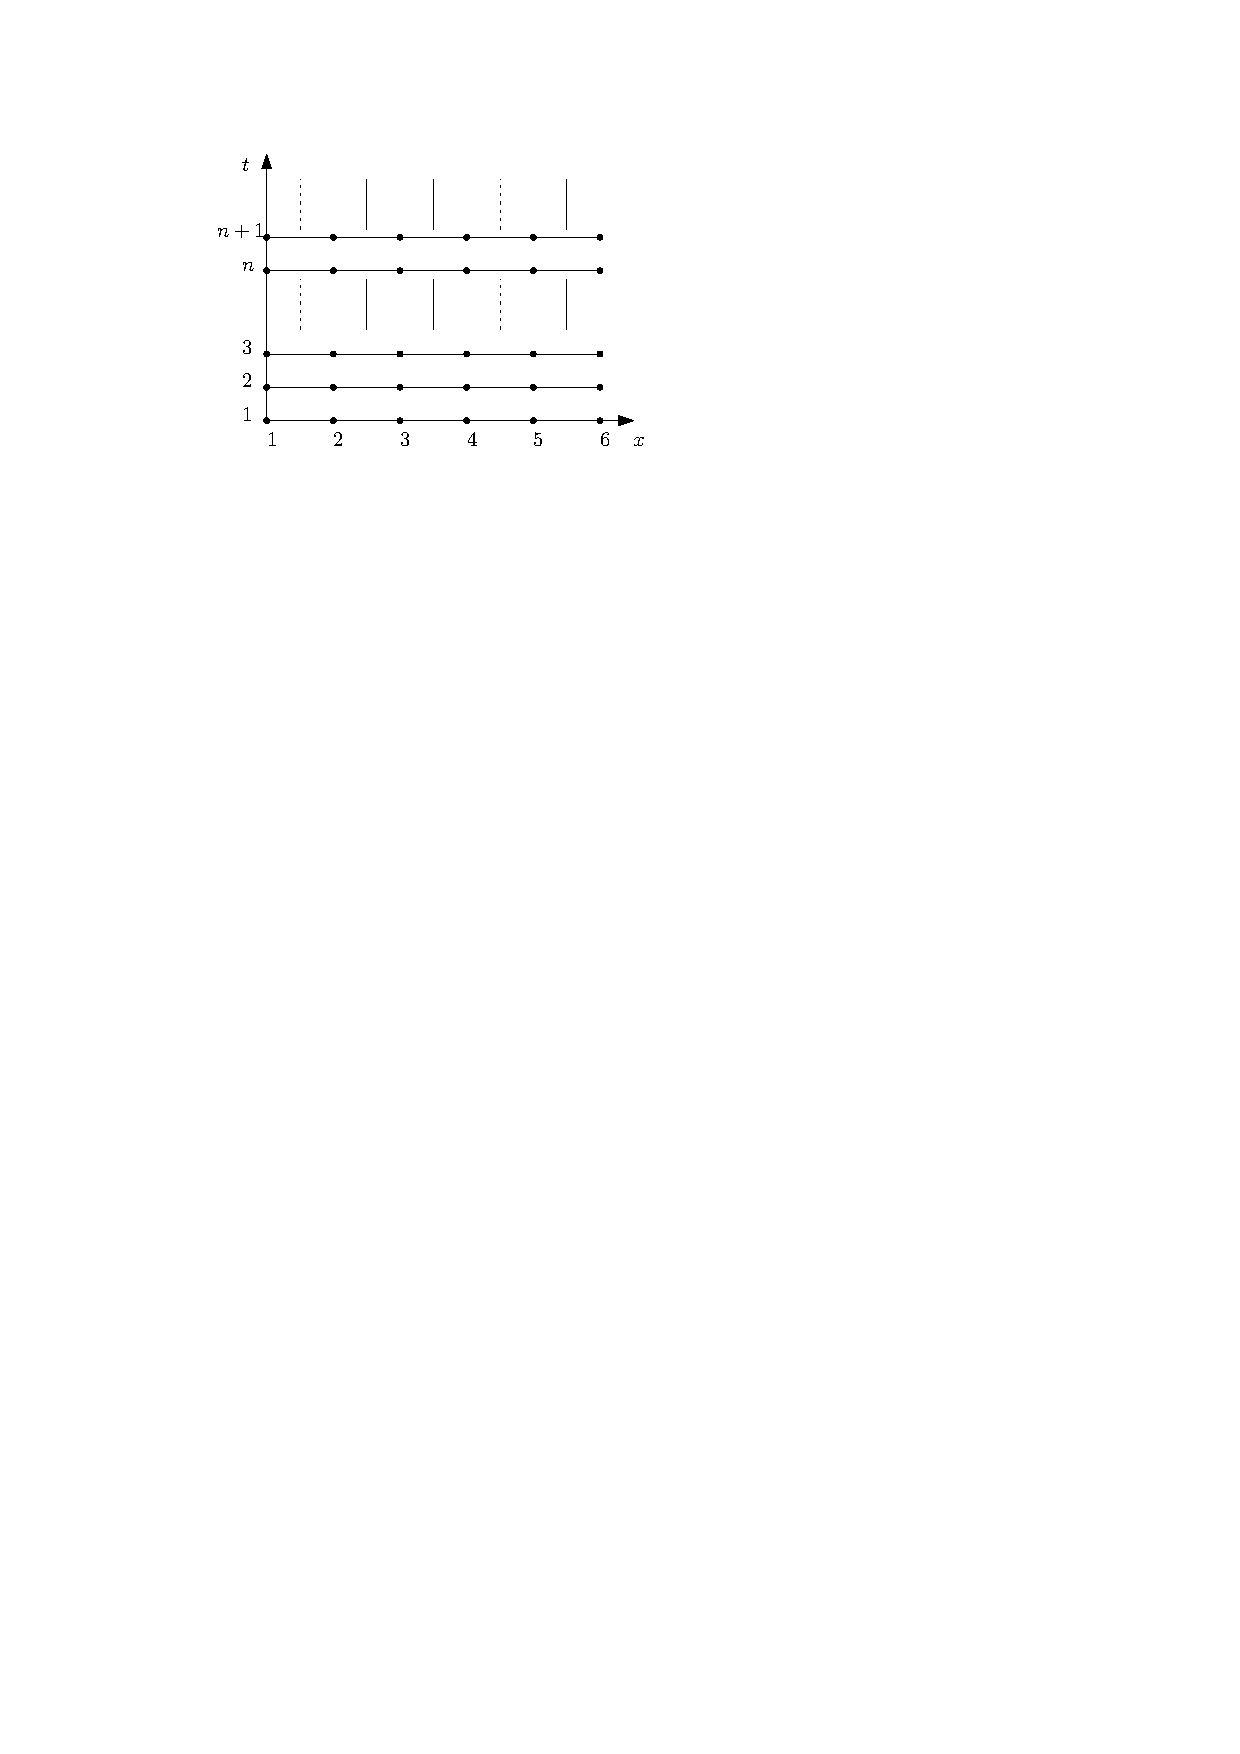
\includegraphics{BD1dht.pdf}
  \caption{求解网格系统}
  \label{FgBD_1dht_grid}
\end{figure}

初始时刻对应第一个时间层,在该层中所有网格节点上的温度值$T_{i}^{1}$均为已知量,第二个时间层
各网格节点上的差分方程如下:
\begin{equation}
\begin{aligned}
  T_{2}^{2} = 
  T_{2}^{1} 
  +
  \alpha\frac{\Delta t}{(\Delta x)^{2}}
  (T_{3}^{1}-2T_{2}^{1}+T_{1}^{1})
  \\
  T_{3}^{2} = 
  T_{3}^{1} 
  +
  \alpha\frac{\Delta t}{(\Delta x)^{2}}
  (T_{4}^{1}-2T_{3}^{1}+T_{2}^{1})
\\
  T_{4}^{2} = 
  T_{4}^{1} 
  +
  \alpha\frac{\Delta t}{(\Delta x)^{2}}
  (T_{5}^{1}-2T_{4}^{1}+T_{3}^{1})
  \\
  T_{5}^{2} = 
  T_{5}^{1} 
  +
  \alpha\frac{\Delta t}{(\Delta x)^{2}}
  (T_{6}^{1}-2T_{5}^{1}+T_{4}^{1})
\end{aligned}
\end{equation}

当第$n$层时间所有网格节点上的温度值$T_{i}^{n}$均为已知量时,下一个时间层,即
$n+1$层,各网格节点上的差分方程如下:
\begin{equation}
\begin{aligned}
  T_{2}^{n+1} = 
  T_{2}^{n} 
  +
  \alpha\frac{\Delta t}{(\Delta x)^{2}}
  (T_{3}^{n}-2T_{2}^{n}+T_{1}^{n})
  \\
  T_{3}^{n+1} = 
  T_{3}^{n} 
  +
  \alpha\frac{\Delta t}{(\Delta x)^{2}}
  (T_{4}^{n}-2T_{3}^{n}+T_{2}^{n})
\\
  T_{4}^{n+1} = 
  T_{4}^{n} 
  +
  \alpha\frac{\Delta t}{(\Delta x)^{2}}
  (T_{5}^{n}-2T_{4}^{n}+T_{3}^{n})
  \\
  T_{5}^{n+1} = 
  T_{5}^{n} 
  +
  \alpha\frac{\Delta t}{(\Delta x)^{2}}
  (T_{6}^{n}-2T_{5}^{n}+T_{4}^{n})
\end{aligned}
\end{equation}
依此类推,即可求出各时间层上各网格节点上的温度值。表\ref{TbBD_1dht_result1}列出
了详细的计算结果。
\begin{table}[h!]
  \begin{center}
  \caption{一维非稳态热传导方程计算结果(显式方法$\Delta t=1\mathrm{s}$)}
  \label{TbBD_1dht_result1}
  \begin{tabular}{|c|r|r|r|r|r|r|r|r|r|r|r|}
    \hline
 & t=0 & t=1s & t=2s & t=3s & t=4s & t=5s & t=6s & t=7s & t=8s & t=9s & t=10s
 \\
  \hline
x=0 & 0 & 0 & 0 & 0 & 0 & 0 & 0 & 0 & 0 & 0 & 0
\\
    \hline
x=1m & 0 & 0.00  & 0.00  & 0.00  & 3.13  & 3.13  & 5.47  & 5.47  & 7.03  & 7.03
     & 8.06  
     \\
    \hline
x=2m & 0 & 0.00  & 0.00  & 6.25  & 6.25  & 10.94  & 10.94  & 14.06  & 14.06  &
16.11  & 16.11  
\\
    \hline
x=3m & 0 & 0.00  & 12.50  & 12.50  & 18.75  & 18.75  & 22.66  & 22.66  & 25.20
     & 25.20  & 26.86 
     \\
    \hline
x=4m & 0 & 25.00  & 25.00  & 31.25  & 31.25  & 34.38  & 34.38  & 36.33  & 36.33
     & 37.60  & 37.60 
     \\
    \hline
x=5m & 50 & 50 & 50 & 50 & 50 & 50 & 50 & 50 & 50 & 50 & 50
\\
    \hline
  \end{tabular}
  \end{center}
\end{table}

改变时间步长$\Delta t=0.1\mathrm{s}$,系数$\alpha\Delta t/(\Delta
x)^{2}=0.05$。重复上述过程,重新求解结果如表\ref{TbBD_1dht_result2}所示。
\begin{table}[h!]
  \begin{center}
    \caption{一维非稳态热传导方程计算结果(显式方法$\Delta t=0.1\mathrm{s}$)}
  \label{TbBD_1dht_result2}
  \begin{tabular}{|c|r|r|r|r|r|r|r|r|r|r|r|}
    \hline
 & t=0 & t=1s & t=2s & t=3s & t=4s & t=5s & t=6s & t=7s & t=8s & t=9s & t=10s
 \\
  \hline
x=0 & 0 & 0 & 0 & 0 & 0 & 0 & 0 & 0 & 0 & 0 & 0
\\
\hline
x=1m & 0 & 0.04  & 0.44  & 1.29  & 2.36  & 3.46  & 4.49  & 5.40  & 6.17  & 6.83  & 7.38 
\\
\hline
x=2m & 0 & 0.45  & 2.23  & 4.59  & 6.94  & 9.07  & 10.91  & 12.46  & 13.77  & 14.85  & 15.75 
\\
\hline
x=3m & 0 & 3.38  & 8.48  & 12.71  & 16.02  & 18.62  & 20.69  & 22.36  & 23.72  & 24.83  & 25.74 
\\
\hline
x=4m & 0 & 16.73  & 24.12  & 28.22  & 30.86  & 32.73  & 34.13  & 35.22  & 36.09  & 36.79  & 37.36 
\\
\hline
x=5m & 50 & 50 & 50 & 50 & 50 & 50 & 50 & 50 & 50 & 50 & 50
\\
    \hline
  \end{tabular}
  \end{center}
\end{table}

改变时间步长$\Delta t=2.5\mathrm{s}$,系数$\alpha\Delta t/(\Delta
x)^{2}=1.25$。重复上述过程,重新求解结果如表\ref{TbBD_1dht_result3}所示
。
\begin{table}[h!]
  \begin{center}
    \caption{一维非稳态热传导方程计算结果(显式方法$\Delta t=2.5\mathrm{s}$)}
  \label{TbBD_1dht_result3}
  \begin{tabular}{|c|r|r|r|r|r|}
    \hline
 & t=0 & t=2.5s & t=5s & t=7.5s & t=10s
 \\
  \hline
x=0 & 0 & 0 & 0 & 0 & 0
\\
\hline
x=1m & 0 & 0.00  & 0.00  & 0.00  & 122.07 
\\
\hline
x=2m & 0 & 0.00  & 0.00  & 97.66  & -341.80 
\\
\hline
x=3m & 0 & 0.00  & 78.13  & -156.25  & 615.23 
\\
\hline
x=4m & 0 & 62.50  & -31.25  & 207.03  & -443.36 
\\
\hline
x=5m & 50 & 50 & 50 & 50 & 50 
\\
    \hline
  \end{tabular}
  \end{center}
\end{table}

对比前两次的计算结果,表\ref{TbBD_1dht_result3}中数据表明,当系数$\alpha\Delta t/(\Delta
x)^{2}$选取不当时,计算结果中会出现不符合物理定律的数值,比如
$-341.80^{\circ}\!\mathrm{C}$。系数$\alpha\Delta t/(\Delta x)^{2}$如何选取将在下
一节中详细展开。

\subsection{隐式方法}
根据上一节差分格式的知识,式\eqref{EqBD_1dht_de}显然并不是唯一的差分方程。为了解
释隐式方法,我们将$\partial^{2}T/\partial x^{2}$的中心差分格式中分子每一项用第$n$
和$n+1$个时间层的平均值来代替,即
\begin{equation}
  \frac{T_{i}^{n+1}-T_{i}^{n}}{\Delta t}
  =
  \alpha
  \frac{
    \frac{1}{2}(T_{i+1}^{n+1}+T_{i+1}^{n}) +
    \frac{1}{2}(-T_{i+1}^{n+1}-T_{i}^{n}) +
    \frac{1}{2}(T_{i-1}^{n+1}+T_{i-1}^{n}) 
  }{(\Delta x)^{2}}
\end{equation}
这个差分格式被称为Crank-Nicolson格式。当然,这个格式并不是唯一的隐式格式,例如,
将中心差分中分子每一项直接用$n+1$层的代入计算。对上式进行整理,将下一个层的未知量放在等式
左边,已知量放在等式右边,可得
\begin{equation}
  \frac{\alpha\Delta t}{2(\Delta x)^{2}}
  T_{i-1}^{n+1} 
  -
  \left[1+\frac{\alpha\Delta t}{(\Delta x)^{2}}\right]
  T_{i}^{n+1} 
  +
  \frac{\alpha\Delta t}{2(\Delta x)^{2}}
  T_{i+1}^{n+1} 
  =
  -T_{i}^{n}
  -
  \frac{\alpha\Delta t}{2(\Delta x)^{2}}
  (T_{i+1}^{n} - 2T_{i}^{n} + T_{i-1}^{n})
  \label{EqBD_1dht_cr_2}
\end{equation}

为了后续推导的便利,令
\begin{equation}
\begin{aligned}
  &A = \frac{\alpha\Delta t}{2(\Delta x)^{2}} \\
  &B = 1 + \frac{\alpha\Delta t}{(\Delta x)^{2}} \\
  &K_{i} = 
  -T_{i}^{n}
  -
  A(T_{i+1}^{n} - 2T_{i}^{n} + T_{i-1}^{n})
\end{aligned}
\end{equation}
式\eqref{EqBD_1dht_cr_2}可写成
\begin{equation}
  AT_{i-1}^{n+1} - BT_{i}^{n+1} + AT_{i+1}^{n+1} = K_{i}
  \label{EqBD_1dht_ia}
\end{equation}
沿用显式格式使用的网格系统,在第2个时间层节点2,3,4和5上的差分方程将形成如下的线性方程组:
\begin{equation}
\begin{aligned}
  AT_{1}^{2}-BT_{2}^{2}+AT_{3}^{2} = K_{2} \\
  AT_{2}^{2}-BT_{3}^{2}+AT_{4}^{2} = K_{3} \\
  AT_{3}^{2}-BT_{4}^{2}+AT_{5}^{2} = K_{4} \\
  AT_{4}^{2}-BT_{5}^{2}+AT_{6}^{2} = K_{5} \\
\end{aligned}
\end{equation}
注意节点2差分方程中$T_{1}^{2}$和节点5差分方程中$T_{6}^{2}$位于边界节点上,因此这
两个值为已知量,可以移到等式的右边。并令$K_{2}^{\prime}=K_{2} - AT_{1}^{2}$,$K_{5}^{\prime}=K_{5} - AT_{6}^{2}$ 则,上式可写成
\begin{equation}
\begin{aligned}
  -BT_{2}^{2}+AT_{3}^{2} = K_{2}^{\prime}\\
  AT_{2}^{2}-BT_{3}^{2}+AT_{4}^{2} = K_{3} \\
  AT_{3}^{2}-BT_{4}^{2}+AT_{5}^{2} = K_{4} \\
  AT_{4}^{2}-BT_{5}^{2} = K_{5}^{\prime}\\
\end{aligned}
\end{equation}
写成矩阵形式为
\begin{equation}
  \begin{bmatrix}
    -B & A & 0 & 0 \\
    A & -B & A & 0 \\
    0 & A & -B & A \\
    0 & 0 & A & -B \\
  \end{bmatrix}
  \begin{bmatrix}
    T_{2}^{2} \\
    T_{3}^{2} \\
    T_{4}^{2} \\
    T_{5}^{2} \\
  \end{bmatrix}
  =
  \begin{bmatrix}
    K_{2}^{\prime} \\
    K_{3} \\
    K_{4} \\
    K_{5}^{\prime} \\
  \end{bmatrix}
\end{equation}

当$\Delta t=1\mathrm{s}$时,$A=\frac{\alpha\Delta t}{2(\Delta
x)^{2}}=\frac{0.5\times1}{2\times1^{2}}=0.25$,$B=1.5$,第一个时间层各节点上温度
值分别为:$T_{i}^{1}=0, i=1,2,\cdots 5$,$T_{6}^{1}=50.0^{\circ}\!\mathrm{C}$,第二个时间层边界节点
温度值分别为:$T_{1}^{2}=0$,$T_{6}^{2}=50.0^{\circ}\!\mathrm{C}$,各节点差分方程右侧
$K_{i}$为
\begin{equation}
\begin{aligned}
    &K_{2}^{\prime} =
    K_{2} - AT_{1}^{2}
    =
  -T_{2}^{1}
  -
  A(T_{3}^{1} - 2T_{2}^{1} + T_{1}^{1})
  - AT_{1}^{2}
  =
  0
    \\
    &K_{3} 
    =
  -T_{3}^{1}
  -
  A(T_{4}^{1} - 2T_{3}^{1} + T_{2}^{1})
  =
  0
    \\
    &K_{4}
    =
  -T_{4}^{1}
  -
  A(T_{5}^{1} - 2T_{4}^{1} + T_{3}^{1})
  =
  0
    \\
    &K_{5}^{\prime} 
    K_{5} - AT_{6}^{2}
    =
  -T_{5}^{1}
  -
  A(T_{6}^{1} - 2T_{5}^{1} + T_{4}^{1})
  - AT_{6}^{2}
  =
  -25.0
    \\
\end{aligned}
\end{equation}
代入矩阵,可得
\begin{equation}
  \begin{bmatrix}
    -1.5 & 0.25 & 0 & 0 \\
    0.25 & -1.5 & 0.25 & 0 \\
    0 & 0.25 & -1.5 & 0.25 \\
    0 & 0 & 0.25 & -1.5 \\
  \end{bmatrix}
  \begin{bmatrix}
    T_{2}^{2} \\
    T_{3}^{2} \\
    T_{4}^{2} \\
    T_{5}^{2} \\
  \end{bmatrix}
  =
  \begin{bmatrix}
    0 \\
    0 \\
    0 \\
    -25.0 \\
  \end{bmatrix}
\end{equation}
从上式可以解出
\begin{equation}
  T_{2} = 0.08, \quad
  T_{3} = 0.50, \quad
  T_{4} = 2.94, \quad
  T_{5} = 17.16
\end{equation}
重复这一过程,即可求出各时间层上各网格节点上的温度值。表\ref{TbBD_1dht_result4}列出了详细的计算结
果。
\begin{table}[h!]
  \begin{center}
    \caption{一维非稳态热传导方程计算结果(隐式方法$\Delta t=1\mathrm{s}$)}
  \label{TbBD_1dht_result4}
  \begin{tabular}{|c|r|r|r|r|r|r|r|r|r|r|r|}
    \hline
 & t=0 & t=1s & t=2s & t=3s & t=4s & t=5s & t=6s & t=7s & t=8s & t=9s & t=10s
 \\
  \hline
    x = 0m & 0& 0& 0& 0& 0& 0& 0& 0& 0& 0& 0
 \\
  \hline
    x=1m & 0 & 0.08 & 0.47 & 1.26 & 2.31 & 3.41 & 4.44 & 5.35 & 6.13 & 6.79 & 7.35
 \\
  \hline
    x = 2m & 0 & 0.50 & 2.14 & 4.49 & 6.86 & 8.99 & 10.83 & 12.40 & 13.70 & 14.79 & 15.70
 \\
  \hline
    x= 3m & 0 &2.94 & 8.33 & 12.63 & 15.95 & 18.55 & 20.62 & 22.29 & 23.65 & 24.77 & 25.68
 \\
  \hline
    x = 4m & 0 & 17.16 & 24.26 & 28.25 & 30.85 & 32.70 & 34.09 & 35.18 & 36.05 &
    36.75 & 37.33
 \\
  \hline
    x=5m &   50 & 50 & 50 &50 &50 &50 &50 &50 &50 &50 & 50
\\
    \hline
  \end{tabular}
  \end{center}
\end{table}

改变时间步长$\Delta t=2.5\mathrm{s}$,重复上述过程,重新求解结果如表\ref{TbBD_1dht_result5}所示。
\begin{table}[h!]
  \begin{center}
    \caption{一维非稳态热传导方程计算结果(隐式方法$\Delta t=2.5\mathrm{s}$)}
  \label{TbBD_1dht_result5}
  \begin{tabular}{|c|r|r|r|r|r|}
    \hline
 & t=0 & t=2.5s & t=5s & t=7.5s & t=10s
 \\
  \hline
x=0 & 0 & 0 & 0 & 0 & 0
\\
\hline
x=1m & 0 & 0.77  & 3.12  & 5.79  & 7.44
\\
\hline
x=2m & 0 & 2.77  & 8.77  & 13.33 & 15.77
\\
\hline
x=3m & 0 & 9.19  & 19.6 & 22.96  & 25.91
\\
\hline
x=4m & 0 & 30.33  & 32.41  & 36.00  & 37.35
\\
\hline
x=5m & 50 & 50 & 50 & 50 & 50 
\\
    \hline
  \end{tabular}
  \end{center}
\end{table}
对比表\ref{TbBD_1dht_result5}和表\ref{TbBD_1dht_result3}可知,隐式方法在时间步长$\Delta t=2.5\mathrm{s}$时仍然可以获得
合理的解,而显式方法获得的解出现了违反物理定律的解。这表明隐式方法比显式方法更为
稳定。然而,对比两种方法的计算量,显式方法直接求解所需的计算步骤很少,而隐式方法
需要求解线性方程组,特别是当节点数量变大,比如$\Delta x=0.001\mathrm{m}$,甚至更
大时,线性方程组的求解步骤很多。关于线性方程组的求解将在下一章中详细讨论。



\section{相容性、稳定性和收敛性}
对给定的差分方程,当$\Delta x \rightarrow 0$和$\Delta t \rightarrow 0$时,截断误差趋
近于0,差分方程将收敛于原偏微分方程,即
\begin{equation}
  \lim_{\Delta t,\Delta x\rightarrow 0}[\mathrm{PDE} - \mathrm{FDE}] = 0
\end{equation}
式中,PDE为偏微分方程,FDE为差分方程。
这种情况下,偏微分方程的差分方程被认为是\textbf{相容的}。需要注意的是,差分方程
收敛于原偏微分方程,并不等价于差分方程的精确解收敛于偏微分方程的精确解。

还是以一维非稳态热传导方程为例,设$T(x,t)$为偏微分方程的精确解,$T_{i}^{n}$为差
分方程的精确解。当$\Delta x \rightarrow 0$和$\Delta t \rightarrow 0$时,若
\begin{equation}
  \lim_{\Delta t,\Delta x\rightarrow 0}[T(x,t) - T_{i}^{n}] = 0
\end{equation}
则差分方程的精确解收敛于原偏微分方程的精确解,或者说差分方程的精确解是收敛的。

当差分方程与原微分方程是相容的,且差分方程的精确解是收敛的,是否就能保证最后能得
到合理的解了?答案是否定的。差分方程的相容性、收敛性是在$\Delta t$和$\Delta x$趋
近于0时来讨论的。在实际应用中,$\Delta t$和$\Delta x$一定是一个有限大的数,截断
误差不会趋近于0。截断误差的存在将会影响差分方程精确解的精度。此外,无论采用何种
计算手段,受计算精度的影响,差分方程的求解都会引入计算误差。计算误差在计算过程中
会不断步进。如果随着计算过程,计算误差逐渐累积,导致误差过大,使计算结果偏离差分
方程的精确解,这种差分方程就是不稳定的。反之,若计算误差在计算过程中能被控
制在一个可接受的程度,计算结果与精确解的差值符合精度要求,这种差分方程就是稳定的
。本节将重点介绍判定差分方程稳定性的黎曼稳定性分析方法。

离散误差和舍入误差是影响偏微分方程数值解的主要两个误差来源。离散误差是指原偏微分
方程精确解与相应的差分方程的精确解之间存在的误差,也就是差分方程的截断误差,外加
边界条件数值化处理引入的误差。舍入误差是指,在求解差分方程时大量浮点运算过程中,计算
机总是将浮点数按照一定有效位数进行舍入而引入的误差。

令$A$为偏微分方程的精确解,$D$为差分方程的精确解,$N$为真实的计算机求解
差分方程得到的数值解。那么,
\begin{equation}
  \begin{aligned}
  &\mbox{离散误差} = A - D
  \\
  &\mbox{舍入误差} = \epsilon = N - D
  \quad
  \mbox{或}
  \quad
  N = D + \epsilon
  \end{aligned}
  \label{EqBD_Errors}
\end{equation}

为了简化讨论,我们沿用一维非稳态热传导方程,以及上节中显式方法使用的差分方程,
\begin{equation}
  \frac{T_{i}^{n+1}-T_{i}^{n}}{\Delta t}
  =
  \frac{\alpha(T_{i+1}^{n}-2T_{i}^{n}+T_{i-1}^{n})}{(\Delta x)^{2}}
  \tag{\ref{EqBD_1dht_de}}
\end{equation}

显然,式\eqref{EqBD_1dht_de}的数值解$N$必定满足该式,即
\begin{equation}
  \frac{N_{i}^{n+1}-N_{i}^{n}}{\Delta t}
  =
  \frac{\alpha(N_{i+1}^{n}-2N_{i}^{n}+N_{i-1}^{n})}{(\Delta x)^{2}}
  \label{EqBD_1dht_de_N}
\end{equation}

将式\eqref{EqBD_Errors}带入上式,有
\begin{equation}
  \frac{D_{i}^{n+1}+\epsilon_{i}^{n} - D_{i}^{n} - \epsilon_{i}^{n}}{\alpha \Delta t}
  =
  \frac{D_{i+1}^{n}+\epsilon_{i+1}^{n} - 2D_{i}^{n}-2\epsilon_{i}^{n}+D_{i-1}^{n}+\epsilon_{i-1}^{n}}{(\Delta x)^{2}}
  \label{EqBD_1dht_error_n}
\end{equation}

根据定义,$D$为差分方程的精确解,因此它一定是满足差分方程的,即
\begin{equation}
  \frac{D_{i}^{n+1}-D_{i}^{n}}{\alpha\Delta t}
  =
  \frac{D_{i+1}^{n}-2D_{i}^{n}+D_{i-1}^{n}}{(\Delta x)^{2}}
  \label{EqBD_1dht_error_d}
\end{equation}

从式\eqref{EqBD_1dht_error_n}中减去式\eqref{EqBD_1dht_error_d}得:
\begin{equation}
  \frac{\epsilon_{i}^{n+1}-\epsilon_{i}^{n}}{\alpha\Delta t}
  =
  \frac{\epsilon_{i+1}^{n}-2\epsilon_{i}^{n}+\epsilon_{i-1}^{n}}{(\Delta x)^{2}}
  \label{EqBD_1dht_error_e}
\end{equation}
可见,舍入误差$\epsilon$同样也满足差分方程。假定$\epsilon_{i}$是计算过程中某一
阶段的误差。那么,随着求解过程从第$n$层步进到第$n+1$层,误差$\epsilon_{i}$收缩或
尽可能保持一致时,解就是稳定的。反之,如果$\epsilon_{i}$随着求解过程变大,
解就是不稳定的。因此,对于一个稳定解,有
\begin{equation}
\left|
\frac{\epsilon_{i}^{n+1}}{\epsilon_{i}^{n}}
\right|
\le
1
\label{EqBD_Stability}
\end{equation}


根据傅里叶级数理论,舍入误差$\epsilon(x,t)$可以表示为:
\begin{equation}
  \epsilon(x,t) = \sum_{m=-\infty}^{\infty}A_{m}(t)e^{ik_{m}x}
\end{equation}
然而,由于实际问题中空间离散后网格尺寸不能为零。例如,上节使用的网格划分,假定网
格节点数为$N$,那么上式中$m$的取值只能是1到$N/2$,即
\begin{equation}
  \epsilon(x,t) = \sum_{m=1}^{N/2}A_{m}(t)e^{ik_{m}x}
\end{equation}
另外,假定$A_{m}(t)=e^{at}$,其中$a$是一个常数。上式可写成
\begin{equation}
  \epsilon(x,t) = \sum_{m=1}^{N/2}e^{at}e^{ik_{m}x}
  \label{EqBD_errors_expression}
\end{equation}

值得注意的是,差分方程本身是一个线性方程,而且误差$\epsilon$满足差分方程。因此,
将误差表达式带入差分方程后,式\eqref{EqBD_errors_expression}中每一项都应该满足差
分方程。因此,我们仅需讨论任一项就可以了。下面以舍入误差的第$m$项展开讨论。
\begin{equation}
  \epsilon_{m}(x,t) = e^{at}e^{ik_{m}x}
  \label{EqBD_errors_m_term}
\end{equation}
将式\eqref{EqBD_errors_m_term}带入式\eqref{EqBD_1dht_error_e},得
\begin{equation}
  \frac{e^{a(t+\Delta t)}e^{ik_{m}x}-e^{at}e^{ik_{m}x}}{\alpha\Delta t}
  =
  \frac{e^{at}e^{ik_{m}(x+\Delta x)}-2e^{at}e^{ik_{m}x}+e^{at}e^{ik_{m}(x-\Delta
  x)}}{(\Delta x)^{2}}
  \label{EqBD_1dht_error_e_fs}
\end{equation}
等式两边同除$e^{at}e^{ik_{m}x}$,可得
\begin{equation}
  \frac{e^{a\Delta t}-1}{\alpha\Delta t}
  =
  \frac{e^{ik_{m}\Delta x}-2+e^{-ik_{m}\Delta x}}{(\Delta x)^{2}}
\end{equation}
移项整理可得
\begin{equation}
e^{a\Delta t} =
1
+
\frac{\alpha \Delta t}{(\Delta x)^{2}}
(e^{ik_{m}\Delta x}+e^{-ik_{m}\Delta x}-2)
\label{EqBD_1dht_e_fs_1}
\end{equation}
根据欧拉公式,有
\begin{equation}
  \cos(k_{m}\Delta x) = 
  \frac{e^{ik_{m}\Delta x}+e^{-ik_{m}\Delta x}}
  {2}
\end{equation}
式\eqref{EqBD_1dht_e_fs_1}可写成
\begin{equation}
e^{a\Delta t} =
1
+
\frac{2\alpha \Delta t}{(\Delta x)^{2}}
(\cos(k_{m}\Delta x)-1)
\label{EqBD_1dht_e_fs_2}
\end{equation}
根据三角函数关系,有
\begin{equation}
  \sin^{2}\frac{k_{m}\Delta x}{2}
  =
  \frac{1-\cos(k_{m}\Delta x)}{2}
\end{equation}
式\eqref{EqBD_1dht_e_fs_2}可写成
\begin{equation}
e^{a\Delta t} =
1
-
\frac{4\alpha \Delta t}{(\Delta x)^{2}}
\sin^{2}\frac{k_{m}\Delta x}{2}
\label{EqBD_1dht_e_fs_3}
\end{equation}

根据式\eqref{EqBD_Stability}
\begin{equation}
\left|
  \frac{\epsilon_{i}^{n+1}}{\epsilon_{i}^{n}}
\right|
  =
  \left|
  \frac{e^{a(t+\Delta t)}e^{ik_{m}x}}{e^{at}e^{ik_{m}x}}
  \right|
=
\left|e^{a\Delta t}\right|
=
\left|
1
-
\frac{4\alpha \Delta t}{(\Delta x)^{2}}
\sin^{2}\frac{k_{m}\Delta x}{2}
\right|
\le 
1
\end{equation}

根据上式,可以定义放大因子$G$。
求解$G\le 1$不等式,可以得到满足稳定性的条件。
\begin{equation}
\left|
1
-
\frac{4\alpha \Delta t}{(\Delta x)^{2}}
\sin^{2}\frac{k_{m}\Delta x}{2}
\right|
=
G
\end{equation}

第一个条件,
\begin{equation}
1
-
\frac{4\alpha \Delta t}{(\Delta x)^{2}}
\sin^{2}\frac{k_{m}\Delta x}{2}
\le 1
\end{equation}
化简得,
\begin{equation}
\frac{4\alpha \Delta t}{(\Delta x)^{2}}
\sin^{2}\frac{k_{m}\Delta x}{2}
\ge
0
\end{equation}
由于,$4\alpha\Delta t/(\Delta x)^{2}$中各项始终为正,因此该不等式是无条件满足的
。

第二个条件,
\begin{equation}
1
-
\frac{4\alpha \Delta t}{(\Delta x)^{2}}
\sin^{2}\frac{k_{m}\Delta x}{2}
\ge -1
\end{equation}
从上式可以得到,要满足稳定性条件,系数$\alpha\Delta t/(\Delta x)^{2}$必须满足的
条件为:
\begin{equation}
\frac{\alpha \Delta t}{(\Delta x)^{2}}
\le
\frac{1}{2}
\end{equation}

差分方程的相容性、收敛性和稳定性对数值解影响显著。根据数学理论,当差分方程的相容
性满足后,若差分方程是稳定性的,那么收敛性自动满足。因此,在推导差分方程过程中,
我们的重点放在相容性和稳定性上。
